%!TEX TS-program = pdflatex
% dissertation.tex -- main dissertation file
%
% Wisconsin dissertation template
% Copyright (c) 2008-2009 William C. Benton.  All rights reserved.
%
% This program can redistributed and/or modified under the terms
% of the LaTeX Project Public License Distributed from CTAN
% archives in directory macros/latex/base/lppl.txt; either
% version 1 of the License, or (at your option) any later version.
%
% This program includes other software that is licensed under the
% terms of the LPPL and the Perl Artistic License; see README for details.
%
% You, the user, still hold the copyright to any document you produce
% with this software (like your dissertation).
%

%%% You'll want ``oneside'' for the deposit version, but probably not for any versions that don't need to meet the UW requirements
\documentclass[12pt,oneside,letterpaper]{memoir}
\usepackage{color}
\usepackage{caption}
\usepackage{subcaption}
% preamble.tex -- packages to include
%
% Wisconsin dissertation template
% Copyright (c) 2008 William C. Benton.  All rights reserved.
%
% This program can redistributed and/or modified under the terms
% of the LaTeX Project Public License Distributed from CTAN
% archives in directory macros/latex/base/lppl.txt; either
% version 1 of the License, or (at your option) any later version.
%
% This program includes other software that is licensed under the
% terms of the LPPL and the Perl Artistic License; see README for details.
%
% You, the user, still hold the copyright to any document you produce
% with this software (like your dissertation).

%% You should use natbib
\IfFileExists{natbib.sty}{%
\usepackage{natbib}%
}{}

%% You probably need appendix, if you want appendices
\IfFileExists{appendix.sty}{%
\usepackage{appendix}%
}{}

%% the spacing in memoir is weird, you'll need to use this
\DisemulatePackage{setspace}
\usepackage[onehalfspacing]{setspace}

%% List setup; the ``hanglist`` environment will allow you to have
%% nicely-typeset enumerated lists (i.e. with the numbers hanging in
%% the margins).  You need at least version 2.1 of enumitem.sty.  If
%% you don't have enumitem installed at all, hanglist will just be an
%% alias for enumerate.
\IfFileExists{enumitem.sty}{%
\usepackage[loadonly]{enumitem}[2007/06/30]%
\newlist{hanglist}{enumerate}{1}% 
\setlist[hanglist]{label=\arabic*.}%
\setlist[hanglist,1]{leftmargin=0pt}%
}{%
\newenvironment{hanglist}{\begin{enumerate}}{\end{enumerate}}%
}

%% Comment out any of these that you don't want
\usepackage{amssymb}
\usepackage{amsmath}
\usepackage{amsthm}
%\usepackage{theorem}
\usepackage{hyperref}

\IfFileExists{mathpartir.sty}{%
\usepackage{mathpartir}%
}{}

%%%%% LISTINGS package and setup
\IfFileExists{listings.sty}{%
\usepackage{listings}%
}{}



%% Get rid of ugly borders around PDF hyperlinks (e.g. for cross-references, bib entries, or URLs)
\hypersetup{pdfborder = 0 0 0}

%% You want microtype.
\IfFileExists{microtype.sty}{%
\usepackage[protrusion=true,expansion=true]{microtype}%
}{}

%\pagestyle{thesisdraft}

% Surround parts of graphics with box
\usepackage{boxedminipage}

%% booktabs (thx to Nate Rosenblum for bringing this beautiful package
%% to my attention)
\IfFileExists{booktabs.sty}{%
\usepackage{booktabs}%
}{}

% This is now the recommended way for checking for PDFLaTeX:
\usepackage{ifpdf}

%% Avoid ugly "Type 3" fonts
\usepackage{lmodern}
\usepackage[LY1]{fontenc}

%% Substitute your favorite serif and sans fonts here....
\IfFileExists{tgpagella.sty}{%
% TeX Gyre pagella, like Palatino
\usepackage{tgpagella}%
}{}

\usepackage[LY1]{eulervm}

\ifpdf
\usepackage[pdftex]{graphicx}
\else
\usepackage{graphicx}
\fi

\usepackage{makeidx}
\makeindex

{\theoremstyle{plain}
\newtheorem{thm}{Theorem}[chapter]
\newtheorem{cor}[thm]{Corollary}
\newtheorem{define}[thm]{Definition}
\newtheorem{exmpl}[thm]{Example}
}
{\theoremstyle{remark}
\newtheorem{rmk}[thm]{Remark}
}

\newtheoremstyle{customsty1}
{3pt}%
{3pt}%
{}% --- body font
{}% --- indent amount
{\bfseries}% --- Theorem head font
{:}% --- Punctuation after head
{.5em}% --- space after head
{}% --- theorem head spec (can be left empty, meaning 'normal')

% Define 'newtheorems' that use ``customsty1''
{\theoremstyle{customsty1} 
}


%%% NB: the ``deposit'' chapter- and page- styles should conform to UW
%%% requirements.  If you are producing a pretty version of your
%%% dissertation for web use later, you will certainly want to make
%%% your own chapter and page styles.

\makechapterstyle{deposit}{%
  \renewcommand{\chapterheadstart}{}
  \renewcommand{\printchaptername}{}
  \renewcommand{\chapternamenum}{}
  \renewcommand{\printchapternum}{\parbox{2em}{\MakeLowercase{\Large\scshape\thechapter{}}} }
  \renewcommand{\afterchapternum}{}
  \renewcommand{\printchaptertitle}[1]{%
  \raggedright\Large\scshape\MakeLowercase{##1}}
  \renewcommand{\afterchaptertitle}{%
  \vskip\onelineskip \hrule\vskip\onelineskip}
}

\makepagestyle{deposit}
 
\makeatletter
 
\renewcommand{\chaptermark}[1]{\markboth{#1}{}}
\renewcommand{\sectionmark}[1]{\markboth{#1}{}}
 
\makeevenfoot{deposit}{}{}{}
\makeoddfoot{deposit}{}{}{}
\makeevenhead{deposit}{\thepage}{}{}
\makeoddhead{deposit}{}{}{\thepage}
\makeatother

%%% set up page numbering for chapter pages to satisfy UW requirements
%%% NB: You will want to delete until the ``SNIP'' mark if you are
%%% making a ``nice'' copy
\copypagestyle{chapter}{plain}
\makeoddfoot{chapter}{}{}{}
\makeevenhead{chapter}{\thepage}{}{}
\makeoddhead{chapter}{}{}{\thepage}
%%% SNIP

%%% bib nonsense
\makeatletter
\newenvironment{wb-bib}[1]{%
  \chapter*{references}
\ifnobibintoc\else 
\phantomsection 
\addcontentsline{toc}{chapter}{References} 
\fi 
\prebibhook
  \begin{bibitemlist}{#1}}{\end{bibitemlist}\postbibhook}

\AtBeginDocument{%
  \@ifpackageloaded{natbib}{% natbib is loaded
    \addtodef{\endthebibliography}{}{\vskip-\lastskip\postbibhook}
    \@ifpackagewith{natbib}{sectionbib}{% with sectionbib option
      \renewcommand{\bibsection}{\@memb@bsec}}%
      {\renewcommand{\bibsection}{\@memb@bchap}}}%
  {}
  \@ifpackagewith{chapterbib}{sectionbib}{%
    \renewcommand{\sectionbib}[2]{}
    \renewcommand{\bibsection}{\@memb@bsec}}{}
}
\makeatother

% defs.tex -- wbepi environment for chapter epigraphs and other useful defs.
%
% Wisconsin dissertation template
% Copyright (c) 2008 William C. Benton.  All rights reserved.
%
% This program can redistributed and/or modified under the terms
% of the LaTeX Project Public License Distributed from CTAN
% archives in directory macros/latex/base/lppl.txt; either
% version 1 of the License, or (at your option) any later version.
%
% This program includes other software that is licensed under the
% terms of the LPPL and the Perl Artistic License; see README for details.
%
% You, the user, still hold the copyright to any document you produce
% with this software (like your dissertation).


%% put lstnewenvironment declarations here, if you're using listings

%% end lstnewenvironment declarations

%% I put convenience definitions that will go in several chapters here

%%%%% begin convenience definitions

\makeatletter
\newcommand{\wb@episource}{}
\newenvironment{wbepi}[1]{\begin{quote}\renewcommand{\wb@episource}{#1}\itshape}{\par\upshape \raggedleft --- \textsc{\wb@episource}\\ \end{quote}}
\makeatother

%%%%% SVN
\IfFileExists{svn-multi.sty}{%
\usepackage{svn-multi}%
%%% Uncomment the second one and comment out the first one if you want
%%% to include subversion revision information in each file.
\newcommand{\vcinfo}{}%
%\newcommand{\vcinfo}{\begin{centering}\fbox{\fbox{\parbox{5in}{Author: \svnauthor\\Revision: \svnfilerev\\Last changed on: \svnfiledate\\URL: \svnkw{HeadURL}}}}\\[1em]\end{centering}}%
}{%
\newcommand{\svnidlong}[4]{}%
\newcommand{\svnfilerev}{}%
\newcommand{\svnauthor}{}%
\newcommand{\svnfiledate}{}%
\newcommand{\svnkw}{}%
\newcommand{\vcinfo}{}%
}

%%%%% end convenience definitions

% thesisdefs.tex

% This is mostly adapted from withesis.cls.  The original copyright
% notice for withesis.cls follows, preceded by two percent signs (%%):

%% withesis.cls
%% LaTeX Style file for the University of Wisconsin-Madison Thesis Format
%% Adapted from the Purdue University Thesis Format
%% Originally by Dave Kraynie
%% Edits by Darrell McCauley
%% Adapted to UW-Madison format by Eric Benedict  (Noted with <EB>)
%% Updated to LaTeX2e by Eric Benedict 24 July 00
%% 
%%=============================================================================
%% Licensed under the Perl Artistic License.
%% see: http://www.ctan.org/tex-archive/help/Catalogue/licenses.artistic.html
%% for more info...
%%=============================================================================

% withesis.cls is available from CTAN.  The modifications to this file
% are also licensed under the Perl Artistic License.

% --wb, 2008

\makeatletter

\newcounter {tocpage}
\newcounter {lofpage}
\newcounter {lotpage}
\newcounter {listofheading}

\newcommand\@thesistitlemedskip{0.2in}
\newcommand\@thesistitlebigskip{0.6in}
\newcommand{\degree}[1]{\gdef\@degree{#1}}
\newcommand{\project}{\gdef\@doctype{A masters project report}}
\newcommand{\prelim}{\gdef\@doctype{A preliminary report}}
\newcommand{\thesis}{\gdef\@doctype{A thesis}}
\newcommand{\dissertation}{\gdef\@doctype{A dissertation}}
\newcommand{\department}[1]{\gdef\@department{(#1)}}

\newenvironment{titlepage}
 {\@restonecolfalse\if@twocolumn\@restonecoltrue\onecolumn
  \else \newpage \fi \thispagestyle{empty}
% \c@page\z@ -- deleted: count title page in thesis
}{\if@restonecol\twocolumn \else \newpage \fi}

\gdef\@degree{Doctor of Philosophy}    %Default is PhD
\gdef\@doctype{A dissertation}         %Default is dissertation

\gdef\@department{(Electrical Engineering)} % Default is Electical Engineering
\gdef\@defensedate{01/01/2100}% Default is a long time from now.
\gdef\@committee{
  Jane Doeverything, Professor, Electrical Engineering\\
  John Dosomethings, Associate Professor, Electrical Engineering\\
  }

\renewcommand{\maketitle}{%
  \begin{titlepage}
%-----------------------------------------------------------------------------
% -- The thesis office doesn't like thanks on title page.  Put it in
% -- the acknowledgments.  This is here so you don't have to change
% -- your titlepage when converting from report style. -> from Purdue, but I
%        left it here since it seems compatible with UW-Madison, Eric
%-----------------------------------------------------------------------------
    \def\thanks##1{\typeout{Warning: `thanks' deleted from thesis titlepage.}}
    \let\footnotesize\small \let\footnoterule\relax \setcounter{page}{1}
    \begin{center}
      {\textbf{\expandafter\expandafter{\@title}}} \\[\@thesistitlebigskip]
       by \\[\@thesistitlemedskip]
      \@author \\[\@thesistitlebigskip]
      \@doctype\ submitted in partial fulfillment of \\
      the requirements for the degree of\\[\@thesistitlebigskip]
      \@degree \\[\@thesistitlemedskip]
      \@department \\[\@thesistitlebigskip]
      at the \\[\@thesistitlemedskip]
      UNIVERSITY OF WISCONSIN--MADISON\\[\@thesistitlemedskip]
      \@date
    \end{center}
    \hspace*{-0.7in}Date of final oral examination: \@defensedate \\[\@thesistitlemedskip]
    \hspace*{-0.7in}The dissertation is approved by the following members of the 
    Final Oral Committee:\\
    \@committee
  \end{titlepage}
  \setcounter{footnote}{0}
  \setcounter{page}{1} %title page is NOT counted
  \let\thanks\relax
  \let\maketitle\relax \let\degree\relax \let\project\relax \let\prelim\relax
  \let\department\relax
  \gdef\@thanks{}\gdef\@degree{}\gdef\@doctype{}
  \gdef\@department{}
  %\gdef\@author{}\gdef\@title{}
}


%=============================================================================
% ABSTRACT
%=============================================================================
% The abstract should begin with two single-spaced lines describing
% the author and title in a standard format.  After these lines comes
% the standard abstract.
%=============================================================================
\def\abstract{
  \chapter*{Abstract}
  \addcontentsline{toc}{chapter}{Abstract}
  \relax\markboth{Abstract}{Abstract}}
\def\endabstract{\par\newpage}


%=============================================================================
% UMI ABSTRACT
%=============================================================================
% The UMI abstract should begin with the author and title in a standard format.
% After the author comes the advisor and university. After these lines comes
% a bunch of double spaced text to make up the standard abstract.
% After the abstract, the advisor's approval signature follows.
% This page is not numbered and is delivered seperately to the thesis office.
%=============================================================================

\def\advisortitle#1{\gdef\@advisortitle{#1}}
\def\advisorname#1{\gdef\@advisorname{#1}}
\gdef\@advisortitle{Professor}
\gdef\@advisorname{Cheer E.\ Place}

\def\umiabstract{
             \thispagestyle{empty}
                  \addtocounter{page}{-1}
                \begin{center}
                  {\textbf{\expandafter\uppercase\expandafter{\@title}}}\\
                  \vspace{12pt}
                  \@author \\
                  \vspace{12pt}
                  Under the supervision of \@advisortitle\ \@advisorname\\
                  At the University of Wisconsin-Madison
                \end{center}
}

\def\endumiabstract{\vfill \hfill\@advisorname\par\newpage}


%============================================================================
% VERBATIMFILE
%============================================================================
% \verbatimfile{<filename>}    for verbatim inclusion of a file
% - Note that the precise layout of line breaks in this file is important!
% - added the \singlespace - EB
%============================================================================
\def\verbatimfile#1{\begingroup \singlespace
                    \@verbatim \frenchspacing \@vobeyspaces
                    \input#1 \endgroup
}


%=============================================================================
% SEPARATOR Pages
%   Creates a blank page with a text centered horizontally and vertically.
%   The page is neither counted nor numbered.
%   These pages are required in the thesis format before sections such
%   as appendices, vita, bibliography, etc.
%=============================================================================
\def\separatorpage#1{
  \newpage
  \thispagestyle{empty}
  \addtocounter{page}{-1}
  \null
  \vfil\vfil
  \begin{center}
    {\textbf{#1}}
  \end{center}
  \vfil\vfil
  \newpage}


%=============================================================================
% COPYRIGHTPAGE
%=============================================================================
% The copyright must do the following:
% - start a new page with no number
% - place the copyright text centered at the bottom.
%=============================================================================
\def\copyrightpage{
  \newpage
  \thispagestyle{empty}    % No page number
  \addtocounter{page}{-1}
  \chapter*{}            % Required for \vfill to work
  \begin{center}
   \vfill
   \copyright\ Copyright by \@author\ \@date\\
   All Rights Reserved
  \end{center}}


%=============================================================================
% GLOSSARY
%=============================================================================
% The glossary environment must do the following:
% - produce the table of contents entry for the glossary
% - start a new page with GLOSSARY centered two inches from the top
%=============================================================================
\def\glossary{
  \chapter*{GLOSSARY}
  \addcontentsline{toc}{chapter}{Glossary}}
\def\endglossary{\par\newpage}

%=============================================================================
% NOMENCLATURE
%=============================================================================
% The nomenclature environment must do the following:
% - produce the table of contents entry for the nomenclature section
% - start a new page with NOMENCLATURE centered two inches from the top
%=============================================================================
\def\nomenclature{\separatorpage{DISCARD THIS PAGE}
  \chapter*{Nomenclature}
  \addcontentsline{toc}{chapter}{NOMENCLATURE}}
\def\endnomenclature{\par\newpage}

%=============================================================================
% CONVENTIONS
%=============================================================================
% The conventions environment must do the following:
% - produce the table of contents entry for the nomenclature section
% - start a new page with CONVENTIONS centered two inches from the top
%=============================================================================
\def\conventions{\separatorpage{DISCARD THIS PAGE}
  \chapter*{Conventions}
  \addcontentsline{toc}{chapter}{CONVENTIONS}}
\def\endconventions{\par\newpage}


%=============================================================================
% COLOPHON
%=============================================================================
% The colophon environment must do the following:
% - produce the table of contents entry for the nomenclature section
% - start a new page with COLOPHON centered two inches from the top
%=============================================================================
\def\colophon{\separatorpage{DISCARD THIS PAGE}
  \chapter*{Colophon}
  \addcontentsline{toc}{chapter}{Colophon}}
\def\endcolophon{\par\newpage}

%=============================================================================
% LIST OF SYMBOLS
%=============================================================================
% The list of symbols environment must do the following:
% - produce the table of contents entry for the list of symbols section
% - start a new page with LIST OF SYMBOLS centered two inches from the top
%=============================================================================
\def\listofsymbols{\separatorpage{DISCARD THIS PAGE}
  \eject
  \chapter*{LIST OF SYMBOLS}
  \addcontentsline{toc}{chapter}{LIST OF SYMBOLS}}
\def\endlistofsymbols{\par\newpage}

%=============================================================================
% VITA
%=============================================================================
% The vita environment must do the following:
% - produce a separator page with the word vita centered
% - produce the table of contents entry for the vita
% - start a new page with VITA centered two inches from the top
%=============================================================================
\def\vita{
%  \separatorpage{VITA}         % UW doesn't require this EB
  \chapter*{VITA}
  \addcontentsline{toc}{chapter}{VITA}}
\def\endvita{\par\newpage}

%=============================================================================
% ACKNOWLEDGMENTS
%=============================================================================
% The acknowledgments environment must do the following:
% - start a new page with ACKNOWLEDGMENTS centered two inches from the top
%=============================================================================
\def\acks{
  \chapter*{Acknowledgments}
}
\def\endacks{\par\newpage}

%=============================================================================
% DEDICATION
%=============================================================================
% The dedication environment must do the following:
% - start a new page
% - center the text vertically
% - include the text in a center environment
%=============================================================================
\def\dedication{
  \newpage
  \null\vfil
  \begin{center}}
\def\enddedication{\end{center}\par\vfil\newpage}

%=============================================================================
% DATE
%=============================================================================
%\def\today{\ifcase\month\or
  %January\or February\or March\or April\or May\or June\or
  %July\or August\or September\or October\or November\or December\fi
  %\space\number\day, \number\year}
\newcount\@testday
\def\today{\@testday=\day
  \ifnum\@testday>30 \advance\@testday by -30
  \else\ifnum\@testday>20 \advance\@testday by -20
  \fi\fi
  \number\day\ \
  \ifcase\month\or
    January \or February \or March \or April \or May \or June \or
    July \or August \or September \or October \or November \or December
    \fi\ \number\year
}


%  Single counter for theorems and theorem-like environments:
\newtheorem{theorem}{Theorem}[chapter]
\newtheorem{assertion}[theorem]{Assertion}
\newtheorem{claim}[theorem]{Claim}
\newtheorem{conjecture}[theorem]{Conjecture}
\newtheorem{corollary}[theorem]{Corollary}
\newtheorem{definition}[theorem]{Definition}
\newtheorem{example}[theorem]{Example}
\newtheorem{figger}[theorem]{Figure}
\newtheorem{lemma}[theorem]{Lemma}
\newtheorem{prop}[theorem]{Proposition}
\newtheorem{remark}[theorem]{Remark}

%=============================================================================
% TABLE OF CONTENTS; LIST OF FIGURES; LIST OF TABLES
%=============================================================================
% In report style, \tableofcontents, \listoffigures, etc. are always
% set in single-column style.  @restonecol is used to keep track of
% whether we need to switch back to double column style after the toc.
%
% The only known problem now is that the first page with the new
% layout is too long.  The problem seems to be that the change to
% textheight doesn't take place on the first page.  Even if it's the
% first line in the table of contents macro.  Presumably the same
% problem also occurs in the lof and lot.
%
% I'm taking a shot at fixing the problem by dropping in a throw-away
% page between the change to the height parameters and the start of
% the chapter.  Isn't elegance wonderful?
%
%=============================================================================

% \def\@tableof#1#2#3#4#5{
% { % limit scope of following declarations!!
%   \@restonecolfalse\if@twocolumn\@restonecoltrue\onecolumn\fi
%   \addtolength{\textheight}{-40pt}       % -24-16
%   \addtolength{\majorheadskip}{-40pt}    % -24-16
%   \addtolength{\headheight}{52pt}        %  36+16
%   \addtolength{\headsep}{-12pt}          % -12
%   \separatorpage{DISCARD THIS PAGE}
%   \chapter*{#1}
%   #5
%   \relax\markboth{#1}{#1}
%   \hbox to \hsize{#2 \hfil Page}
%   \singlespace
%   \setcounter{#3}{0}
%   \setcounter{listofheading}{1}  % change from 0 to 1 by mccauley, 14may93
%   \def\@oddhead{\vbox to \headheight{\vspace{4pt}
%     \hbox to \hsize{\hfil\textrm{\thepage}} \vfil
%     \ifnum\value{#3}=1
%       \ifnum\value{listofheading}=2
%         \hbox to \hsize{Appendix\hfil} \vspace{4pt} \fi
%       \ifnum\value{listofheading}=1
%         \stepcounter{listofheading} \fi
%       \hbox to \hsize{#2 \hfil Page}
%     \else
%       \setcounter{#3}{1}
%     \fi}}
%   \def\@evenhead{\vbox to \headheight{\vspace{4pt}
%     \hbox to \hsize{\textrm{\thepage}\hfil} \vfil
%     \ifnum\value{#3}=1
%       \ifnum\value{listofheading}=2
%         \hbox to \hsize{Appendix\hfil} \vspace{4pt} \fi
%       \ifnum\value{listofheading}=1
%         \stepcounter{listofheading} \fi
%       \hbox to \hsize{#2 \hfil Page}
%     \else
%       \setcounter{#3}{1}
%     \fi}}
%   \@starttoc{#4}  \if@restonecol\twocolumn\fi
%   \newpage
% }}
% 
% \def\tableofcontents{\@tableof{TABLE OF CONTENTS}{}{tocpage}{toc}{}}
% 
% \def\listoffigures{
%   \@tableof{LIST OF FIGURES}{Figure}{lofpage}{lof}
%   {\protect\addcontentsline{toc}{chapter}{LIST OF FIGURES}}}
% 
% \def\listoftables{
%   \@tableof{LIST OF TABLES}{Table}{lotpage}{lot}
%   {\protect\addcontentsline{toc}{chapter}{LIST OF TABLES}}}

%=============================================================================
% BIBLIOGRAPHY
%=============================================================================
% The thebibliography environment executes the following commands:
%
%  o start a new 'chapter' with BIBLIOGRAPHY as the heading
%  o produce a separator page for the bibliography
%
%  \def\newblock{\hskip .11em plus .33em minus -.07em} --
%      Defines the `closed' format, where the blocks (major units of
%      information) of an entry run together.
%
%  \sloppy  -- Used because it's rather hard to do line breaks in
%      bibliographies,
%
%  \sfcode`\.=1000\relax --
%      Causes a `.' (period) not to produce an end-of-sentence space.
%=============================================================================
% \altbibtitle
%   The default title for the References chapter is ``LIST OF REFERENCES''
%   Since some people prefer ``BIBLIOGRAPHY'', the command
%   \altbibtitle has been added to change the chapter title.
%   This command does nothing more than change REFERENCES to BIBLIOGRAPHY
%============================================================================
\def\@bibchaptitle{Bibliography}
\def\altbibtitle{\def\@bibchaptitle{Bibliography}}
\def\thebibliography#1{
  %\separatorpage{\@bibchaptitle}
  \global\@bibpresenttrue
  \chapter*{\@bibchaptitle\markboth{\@bibchaptitle}{\@bibchaptitle}}
  \addcontentsline{toc}{chapter}{\@bibchaptitle}
  \vspace{0.375in}    % added to match 4 line requirement
  \interlinepenalty=10000 % added to prevent breaking of bib entries
  \singlespace\list
  {[\arabic{enumi}]}{\settowidth\labelwidth{[#1]}\leftmargin\labelwidth
    \advance\leftmargin\labelsep \usecounter{enumi}}
  \def\newblock{\hskip .11em plus .33em minus -.07em}
  \sloppy
  \sfcode`\.=1000\relax}
\let\endthebibliography=\endlist



\makeatother

\svnidlong{$LastChangedBy$}{$LastChangedRevision$}{$LastChangedDate$}{$HeadURL: http://freevariable.com/dissertation/branches/diss-template/dissertation.tex $} 
\graphicspath{ {./images/} }
\clearpage\pagenumbering{roman}  % This makes the page numbers Roman (i, ii, etc)

\title{Efficient Solver }
\author{Haixiang Liu}
\department{Computer Sciences}

\date{2018}

\begin{document}

%%% Uncomment the following if your .bib contains references that you will not 
%%% explicitly cite, but that should be in the final bibliography:
% \nocite{*}

\ifpdf
\DeclareGraphicsExtensions{.pdf, .jpg, .tif, .png}
\else
\DeclareGraphicsExtensions{.eps, .jpg, .png}
\fi

\maketitle

%% Add \part declarations if you want, but it's not necessary
%\part{Preliminaries}

\svnidlong{$LastChangedBy$}{$LastChangedRevision$}{$LastChangedDate$}{$HeadURL: http://freevariable.com/dissertation/branches/diss-template/frontmatter/frontmatter.tex $}
\vcinfo{}

%%% SOME OF THIS CODE IS ADAPTED FROM THE VENERABLE withesis.cls

% COPYRIGHT PAGE
%  - To include a copyright page use \copyrightpage
\copyrightpage

% DEDICATION
\begin{dedication}
	\emph{Please insert your dedication here.}
\end{dedication}

%% BEGIN PAGESTYLE

%%% You can pick a pagestyle if you want; see the memoir class
%%% documentation for more info.  The default ``deposit'' option meets
%%% the UW thesis typesetting requirements but is probably
%%% unsatisfactory for making a version of your dissertation that
%%% won't be deposited to the graduate school (e.g. for web or a nice
%%% printed copy)

\chapterstyle{deposit}
\pagestyle{deposit}


% ACKNOWLEDGMENTS
\begin{acks}
\begin{wbepi}{David C.~Makinson (1965)}
It is customary for authors of academic books to include in their prefaces statements such as this: ``I am indebted to ... for their invaluable help; however, any errors which remain are my sole responsibility.'' Occasionally an author will go further. Rather than say that if there are any mistakes then he is responsible for them, he will say that there will inevitably be some mistakes and he is responsible for them....

Although the shouldering of all responsibility is usually a social ritual, the admission that errors exist is not --- it is often a sincere avowal of belief. But this appears to present a living and everyday example of a situation which philosophers have commonly dismissed as absurd; that it is sometimes rational to hold logically incompatible beliefs.
\end{wbepi}

Above is the famous ``preface paradox,'' which illustrates how to use the \texttt{wbepi} environment for epigraphs at the beginning of chapters.  You probably also want to thank the Academy.
\end{acks}

% CONTENTS, TABLES, FIGURES
\renewcommand{\printtoctitle}[1]{\chapter*{#1}}
\renewcommand{\printloftitle}[1]{\chapter*{#1}}
\renewcommand{\printlottitle}[1]{\chapter*{#1}}

\renewcommand{\tocmark}{}
\renewcommand{\lofmark}{}
\renewcommand{\lotmark}{}

\renewcommand{\tocheadstart}{}
\renewcommand{\lofheadstart}{}
\renewcommand{\lotheadstart}{}

\renewcommand{\aftertoctitle}{}
\renewcommand{\afterloftitle}{}
\renewcommand{\afterlottitle}{}

\renewcommand{\cftchapterfont}{\normalfont} 
\renewcommand{\cftsectionfont}{\itshape} 
\renewcommand{\cftchapterpagefont}{\normalfont} 
\renewcommand{\cftchapterpresnum}{\bfseries} 
\renewcommand{\cftchapterleader}{} 
\renewcommand{\cftsectionleader}{} 
\renewcommand{\cftchapterafterpnum}{\cftparfillskip} 
\renewcommand{\cftsectionafterpnum}{\cftparfillskip} 

% \captionnamefont{\small\sffamily} 
% \captiontitlefont{\small\sffamily} 

% \renewcommand{\contentsname}{contents}
% \renewcommand{\listfigurename}{list of figures}
% \renewcommand{\listtablename}{list of tables}

\tableofcontents

\clearpage
\listoftables

\clearpage
\listoffigures

\clearpage
% NOMENCLATURE
% \begin{conventions}
% % \begin{description}
% % \item{\makebox[0.75in][l]{term}
% %        \parbox[t]{5in}{definition\\}}
% % \end{description}
% \input{conventions}
% \end{conventions}

%% The UW graduate school no longer wants a UMI abstract page
%% Should you need one for some reason, uncomment the following
%% lines.  Thanks to Matt Fredrikson for reporting this!

% \advisorname{Gottlob Frege}
% \advisortitle{Professor}
% \begin{umiabstract}
%  Numerical simulation of physical phenomenal has long been of the interests in the area of mechanical engineering, physics, and in recent year computer graphics. The research in the field usually falls into two categories: modeling and solver. Research in modeling intends in finding mathematical equations, sometimes with better accuracy, sometimes are easier to solve, that can be used to describe the physical phenomenal. Research in solvers, on the other hand, is to develop algorithms that are able to solve larger equations faster, for iterative approximate solvers, solve to higher accuracy.  This dissertation focus on designing efficient solvers, centering on a novel data structure namely SPGrid, which provides the flexibility of a sparse and adaptive data structure while retains the performance of a uniform grid. Furthermore, it will present the use of modern Same Instruction Multiple Data(SIMD) hardware and heterogenous platforms that exploits their high computation throughputs to saturate memory utility. Finally, the efficiency of those design principles and practices are demonstrated in the Poisson and Linear elasticity solvers.
% \end{umiabstract}

\begin{abstract}
  Numerical simulation of physical phenomenal has long been of the interests in the area of mechanical engineering, physics, and in recent year computer graphics. The research in the field usually falls into two categories: modeling and solver. Research in modeling intends in finding mathematical equations, sometimes with better accuracy, sometimes are easier to solve, that can be used to describe the physical phenomenal. Research in solvers, on the other hand, is to develop algorithms that are able to solve larger equations faster, for iterative approximate solvers, solve to higher accuracy.  This dissertation focus on designing efficient solvers, centering on a novel data structure namely SPGrid, which provides the flexibility of a sparse and adaptive data structure while retains the performance of a uniform grid. Furthermore, it will present the use of modern Same Instruction Multiple Data(SIMD) hardware and heterogenous platforms that exploits their high computation throughputs to saturate memory utility. Finally, the efficiency of those design principles and practices are demonstrated in the Poisson and Linear elasticity solvers.
\end{abstract}

\clearpage\pagenumbering{arabic}

%%% END STUFF TAKEN FROM WITHESIS EXAMPLE FILE


%% Now include the tex files for each chapter, like so (I put these in separate dirs): 
\chapter{Introduction}
In recent years, computation power in workstations has leaped, not by increasing core speed,  but by increment of core count, larger SIMD(same instruction multiple data) width(such as AVX512), deeper level of memory hierarchy(such as MCDRAM in knights landing), and bus interconnected accelerators(such as GPUs). This change of hardwares has opened up new opportunities in re-designing and re-architecting algorithms in numerical simulation that adapts to this paradigm.

This documents presents a set of techniques and algorithms for solving large scale linear equations that emerge from the simulations of physical phenomenal targeted for modern hardwares. They are demonstrated by adapting and redesigning solvers for two specific problems: homogeneous Poisson and heterogeneous linear elasticity, discretized on a Cartesian grid. The solvers presented  in this thesis has enabled billion degrees of freedom (DOF) simulations on a single workstation. Such scale not only provided a stunning level of visual detail and higher accuracy in solution, but also, exposed the limitations of the iterative solvers.

For those discoveries, the last part of the thesis proposes a novel augmented geometric Multigrid solver for linear elasticity that address the slow convergence issue of standard Multigrid preconditioned conjugate gradient solvers on domains with complex geometry.

\section{Thesis}

The progression of computation power of modern processors has shifted towards the direction of more parallelism and more heterogeneous. In pursue of higher resolution simulations, new paradigm for designing solvers are needed to take advantage of this shift. This document uses concrete designs of two solvers to demonstrates this new paradigm. The solvers are benchmarked and compared with the theoretical throughput of the platform to illustrate their efficiency.

At achieving higher resolution, the limitation of existing numerical methods will be explored. This document will also propose new algorithms that addresses those limitations. 

\section{Motivation}

Physics based simulation originated in the field of engineering. Some examples are: Air dynamic simulation has been wildly used in aircraft design. The simulation of elasticity has been employed for designs of large scale structures. In recent years, physics based simulation has also been applied in the field of computer graphics. The simulation of smoke and water has been ubiquitous in special effects. The soft body simulation has also made into the standard animation pipelines.

The scale of simulation is important for two major reasons: first, large scale simulation is important when evaluating the convergence of the solution for the purpose pf validation. Numerical simulations discretize continuous equations and solve them with a given resolution. At the limit of refinement, the discretized solution will converge to the continuous one. The ability of going higher resolution in simulation can be used to validate that the discretized solutions' convergence to the continious problem. and used to extrapolate the continuous solution. Second, large scale can simulate more detailed structures. Those details are not only for visual richness, but also significant for finding solutions for complex structures.

To increase the scale of simulation, traditionally it was rely upon frequency scaling of CPU core speed. But in the past 10 years, such scaling has come to a halt. The exponential computation power growth on CPU has been achieved through increment of core counts and wider data level parallelism width. In the meanwhile, computation accelerators (GPUs, Intel Xeon Phi) has emerged as potent computation units that provides fast memory bandwidth and significant amount of computation FLOPS( Floating Point Operations per Second) with the trade off that they usually has a smaller memory size, less integer operations, and slower unaligned random memory assess due to the lack of large memory cache.

Inspired by the change in modern hardware, this document takes examples to demonstrate efficient numerical solvers in the context of modern hardware. Sometimes it requires careful re-engineering existing algorithms combined with a novel data structure to achieve a faster and more memory efficient solver, and sometimes it requires a brand new algorithm that takes the hardware heterogeneity into consideration to avoid hardware bottleneck.

\section{Contributions}

\paragraph{Data-Level Parallelism for Simulation Using SIMD}  Techniques that utilize SIMD instructions, not only on accelerators, but also on AVX-enabled CPUs are presented. The main challenge in SIMD programming is to assess memory in alignment. The document also presents the cases that when aligned memory assess is difficult to achieve, SIMD can also be used for stack allocated data to maximize computation density.

\paragraph{A Domain Decomposition Algorithm Targeting Multi-Accelerator Computation Platform} Design of a homogeneous Poisson solver that utilize multi-accelerator equipped compute platforms. A multi-accelerator equipped compute platform can features an order of magnitude higher aggregate compute FLOPS and memory bandwidth. But the inter-accelerator communication is carried on data buses(such as PCI-E) that have both low bandwidth and high latency. An novel domain decomposition algorithm is presented that targets to minimize the frequency and amount of data that is communicated between across accelerators.

\paragraph{Examination Of Numerical Limit At High Resolution Simulation and Mix Precision Scheme} At high simulation resolution, the discrete differential operators start to exhibit larger numerical cancellation error. To avoiding the full cost of double precision, a mix precision scheme is proposed to achieve double precision accuracy while retain the most of the computation in single precision.

\paragraph{A Stencil-Aware Geometric Multigrid Algorithm For Linear Elasticity} One of the advantage of high resolution simulation is the amount of detail that is capable of capturing. But those complex geometrical details can severely impair the convergence of existing multi-linear interpolated Multigrid solver convergence. To address this convergence problem for high resolution linear elasticity simulation, a stencil-aware geometric Multigrid algorithm is proposed that can reduce residual by approximately half every itertation even with the most irregular domains.

\section{Sparse Paged Grid as Data Structure} 
There are many ways to discretize a continuous simulation domain, the three most common ones are Cartesian grids representations, conforming mesh representation and particle representation. In this work, a Cartesian grid based data structure named Sparse Paged Grid (SPGrid) \cite{setaluri2014spgrid} for the following reasons:
\begin{itemize}
	\item a Cartesian grid based discretization is regular. Every degree of freedom(DOF) is connected to the same number of DOF with the same geometric offsets. Such regularity makes data level parallelism and utilizing SIMD instructions significantly easier in comparison to other representation.
	\item SPGrid utilized the virtual memory for sparsity  management, which eliminates additional memory address look up which are needed for traditional sparse data structure. It's access cost is close to a cache optimized dense uniform grid.
\end{itemize}
The biggest draw back of using a Cartesian grid discretization is the inaccurate capture of the boundary of the domain. Though this document itself does not deal with this inaccuracy. But there are many previous works that targeted this limitation in both the field of elasticity[\cite{zhu2012second}], and fluid simulation[\cite{sethian2003level}]. 

\section{Outline}
The remaining chapters of the documents is divided as the following. Chapter \ref{Chapter:Solver} provides an overview of state of the art numerical solvers for simulation, specific a class of solvers namely Multigrid methods. Chapter \ref{Chapter:DD} presents a novel domain decomposition method that utilizes multi-accelerator equipped platform for Poisson equations. Chapter \ref{Chapter:Elasticity} presents a SIMD optimized solver for linear elasticity that designed for minimizing memory footprint and maximizing computational throughput of modern hardware. Chapter \ref{Chapter:BBMG} presents an augmented geometric Multigrid method that overcomes the slow convergence issue when solving linear elasticity problems with complex domain using traditional methods.  Chapter \ref{Chapter:Future} concludes this document by revisiting the contributions brought by this dissertation and looks into the future work leaded by the limitation of the methods presented.

\chapter{Numerical Solvers in Physics Based Simulation} \label{Chapter:Solver}
In the pipeline of physics based simulation, the complexity of majority of the stages are simply $O(N)$, where $N$ is the number of unknowns, while the complexity of the solve stage can be as much as $O(N^2)$. For high resolution simulation, the solve stage can often take over 90\% of the simulation time. There are two major categories of numerical solvers, direct solvers and iterative solvers. 

Direct solvers provide solution at the precision of the numerical limit, and they generally operates in sparse matrix format (for instance Compressed Sparse Column). Therefore they can be used in arbitrary discretization and problems, but they have the minimal cost of $O(N^2)$ and memory footprint of $O(N^{\frac{4}{3}})$ or higher. This super-linear cost makes direct solvers infeasible for high resolution simulations. But for small scale simulations, direct solver algorithms such as Cholesky factorization are attractive for their accuracy and robustness. 

Iterative solvers, on the other hand, as the name suggests, provides a solution that converges to the exact solution with each iteration. Some iterative solvers, such as Conjugate Gradient Method[\cite{nocedal2006conjugate}] and Generalized Minimal Residual algorithm\cite{saad1986gmres}], mathematically speaking, can achieve the exact solution at the $N$th iteration. At the cost of $O(N)$ per iteration, it will give the exact solution with $O(N^2)$ cost. But in practice, due to numerical drift, those algorithm will require restarts for large problems, and can't achieve the exact solution to numerical limit. 

For large problems, an iterative solver is preferred over direct solver for two major reasons: 1. the memory footprint of an iterative solver is usually $O(N)$, which allows larger problems to fit into memory. 2. Though iterative solve can potentially takes longer to achieve solution at numerical limit, the option to terminate early in exchange for an approximate solution is attractable when computation time is limited. But at higher and higher resolution, iterative solvers can take considerably longer to converge and sometimes even stagnate (See results in Chapter \ref{Chapter:Elasticity}). If terminates too early, the poorly approximated solution can lead to unphysical results, due to that the solution can not satisfies the governing equation.

\section{Multigrid Method Overview}
Multigrid method was proposed in work [\cite{brandt1977multi}]. The multigrid fundamental idea lies as follows: we start with a set of grids $G^0$,$G^1$,...,$G^M$, which are all discretization of the same domain $\Omega$. With higher level consists of a coarser elements. In our uniform grid discretization, int 1D, if the nodes in $G^0$ lies on points $(0,h,2h,3h,4h...)$. We can construct the next level $G^1$ as nodes on points $(0,2h,4h,6h,8h...)$.

If our continuous PDE of the boundary value problem takes the form:
\begin{equation}
LU(x) = F(x)\text{, in }\Omega,  \Lambda U(x) = \Phi(x)\text{, on the boundary }\partial\Omega
\end{equation}
Here, $L$ and $\Lambda$ are the differential operators that are on the interior of the domain and the boundary respectively. $U(x)$ is the solution we seek. $F(x)$ and $\Phi(x)$ are the loading condition that are given. We can now write the discretized PDE at each level $k$ as:
\begin{equation}\label{equ:mg_operator}
L^kU^k(x) = F^k(x)\text{, for} x \in G^k,  \Lambda^k U^k(x) = \Phi^k(x)\text{, for} x\in\partial G^k 
\end{equation}
Now, $L^k$ and $\Lambda^k$ are linear operators and can be perceived as matrices. We are interested in acquiring the solution at the finest level. The main idea is, if at $k$th level, the solution $U^k(x)$ is a good approximation to the continuous $U(x)$. We can use the $k$th level solution as a potent guess for the $k-1$ level. Then apply a correction routine called \textbf{smoother} that is $O(|G^{k-1}|)$ cost to bring the guess close to solution. This process, sometimes refers to as V-cycle or W-cycle, is repeated until $U^0(x)$ is considered close enough to the solution. 

Multigrid has the property that each iteration can reduce the error by at least a constant factor $W$. That is $\frac{|\mathbf{e}_{i+1}|}{|\mathbf{e}_{i}|}<W$. Here we take $|\mathbf{e}|$ as the infinite norm of $\mathbf{e}$. What the value of $W$ is depends on the PDE, how the discretization of each level is constructed, and how potent the smoother is. The convergence property of multigrid will  be elaborate more in later section. But we can see that if we seek to reduce the error by 6 orders of magnitude, we will need $-\log_W 10^6$ iterations to converge, which is a constant. For instance if $W = 0.5$, it will take at most 20 iterations to converge. But, of course, in bad cases, for instance, when $W = 0.99$, it will take about 1400 iterations.

Now we have introduced some fundamental multigrid concepts, let's take a deep look at multigrid implementations.
\section{Construction of the Hierarchy}
For constructing the discretized hierarchal operators in equations \ref{equ:mg_operator}, there are two common ways, geometric coarsening and Galerkin coarsening. In work [\cite{zhu2010efficient}], [\cite{mcadams2010parallel}], geometric coarsening was used to construct hierarchal operators. For the domain decomposition solver, geometric coarsening based multigrid is used as it's building block, see Chapter \ref{Chapter:DD}. 

But in many cases, only the top level operator is provided to the solver, and the underlining PDE is inaccessible, re-discretization of the PDE with a coarser grid(or mesh) is not an option, in those cases, Galerkin coarsening is usually used for constructing the hierarchy, such as in work [\cite{dendy1982black}], [\cite{brezina2001algebraic}], and [\cite{dohrmann2007interpolation}]. This is also our method for the multigrid construction in our SIMD-optimized solver for topology optimization.  

When the underlining PDE is unavailable, there is the possibility to acquire the geometric coarsened operator through homogenization of Galerkin coarsened operator which is demonstrated in work [\cite{moulton1998black}]. But this is aspect is not the focus of this work. Therefore I will leave out here the discussion of homogenization.
\section{Geometric Coarsening}
Geometric coarsening refers to the method of constructing the Multigrid hierarchy through re-discretization with different grid size. It has been proven effective for both homogeneous Poisson[\cite{mcadams2010parallel}] and homogeneous elasticity[\cite{zhu2010efficient}]. Here I will take finite difference Poisson discretization as an example to demonstrates the geometric coarsening principles and its limitation. For more details, I would refer the reader to the work[\cite{mcadams2010parallel}].

The continuous PDE of homogeneous Poisson can be written as:
\begin{equation}
\Delta p\mathbf{x} = f\mathbf{x} \text{ in } \Omega \in \mathcal{R}^3
\end{equation}
$$
p(\mathbf{x}) = \alpha(\mathbf{x}) \text{ on } \Gamma_D\text{, } p_n(\mathbf{x}) = \beta(\mathbf{x}) \text{ on } \Gamma_N
$$
The finite difference discretization on a uniform grid of size $h$, samples points we denote as $\{i,j,k\} \in \mathcal{N}^3$ that corresponding to geometric location $\{ih,jh,kh\} \in \Omega$. The finite difference discretized operator for the interior can be written as:
\begin{equation}
\sum_{i',j',k'\in \mathcal{N}_{[i,j,k]}}\frac{p_{[i',j',k']}-p_{[i,j,k]}}{h^2} = f_{[i,j,k]}
\end{equation}
$$
\mathcal{N}_{[i,j,k]} = \{(i\pm1,j,k),(i,j,k\pm1),(i,j,k\pm1)\}
$$
It is a 2nd order accurate discretization as we can write:
$$
\frac{\partial^2 p}{\partial x^2}(x_0) = \frac{p(x_0)-p(x_0)}{h^2} + O(h^2)
$$
As for boundary conditions, either Nuemann/nature boundary or Dirichlet/essential boundary, we can discretize the operator as shown in Figure ~\ref{fig:PoissonBoundary}. It is only 2nd order accurate, if the boundary condition is perfect aligned with cell. But generally multigrid is used as preconditioner. For that purpose, this discretization is proven to be sufficient for preconditioner even with non-cell align boundaries[\cite{aanjaneya2017power}]. 
\begin{figure}[t]
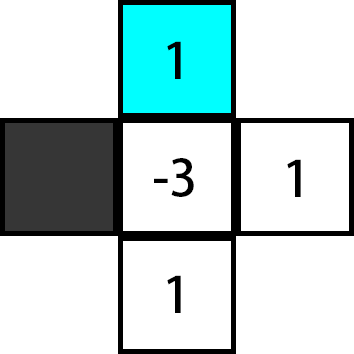
\includegraphics[width=4cm]{Poisson_Stencil}
\centering
\label{fig:PoissonBoundary}
\caption{A finite difference Poisson stencil on the boundary. White cells are interiors cell, i.e. they are degrees of freedom. Blue cell are Dirichlet condition, or essential conditions, that their value are prescribed. Grey cells are exterior cells that are not part of the domain $\Omega$. The face between gray and white cell describes a Nuemann condition, or a nature boundary.}
\end{figure}

But even though we may assume that the boundary conditions are cell aligned at the finest level, this may not holds true for the coarse levels, when the cell size doubles. Figure ~\ref{fig:GeometricCoarsening} demonstrates the heuristic for coarsening boundary conditions. Note that after coarsening, the coarse level discretization may not be of the same order of accuracy to the continuous PDE as the finest level at the boundaries. This inconsistent boundary conditions break the principle that the each level of the multigrid hierarchy should be the discretization of the \textbf{same} continuous PDE. But to compensate this discrepancy, we can introduce additional boundary smoothing to stabilize the multigrid.
\begin{figure}[t]
\centering
\begin{minipage}{.5\textwidth}
  \centering
  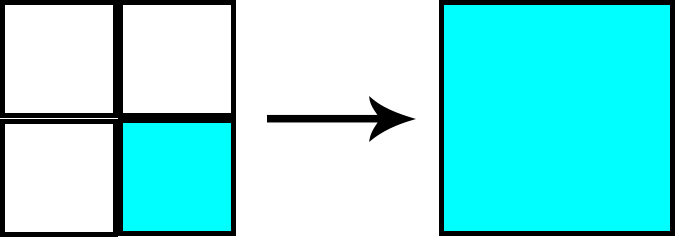
\includegraphics[width=.8\linewidth]{Dirichlet_Coarsening}
\end{minipage}%
\begin{minipage}{.5\textwidth}
  \centering
  
\includegraphics[width=.8\linewidth]{Nuemann_Coarsening}
\end{minipage}
  \caption{Geometric coarsening of the simulation domain. Left: if one of the cells is Dirichlet cell, we will coarsen it as Dirichlet cell at the coarse level, Right: otherwise if one of the cells is interior cell, we will coarsen it as interior cell at the coarse level}
  \label{fig:GeometricCoarsening}
\end{figure}
\section{Garlerkin Coarsening}
Galerkin coarsening, also sometimes refers to algebraic coarsening, is usually the preferred method for handling complex geometries or heterogeneous domains. It was summarized in work [\cite{brandt1986algebraic}]. Many algebraic algorithms, assumes only the top level linear operator is available in matrix form. In such case, the first step of the algorithm is to select the coarse grid DOF based on the matrix given. In this dissertation, we choose the coarsened DOF the same way as in geometric multigrid, that is, coarse DOF coincide with every other fine DOF in each dimension. If readers are interested in the coarse grid selection, I will direct to work [\cite{vanvek1996algebraic}][\cite{brandt1986algebraic}].

After the coarse grid selection, a \textbf{prolongation} operator is constructed. It is a linear operator that interpolates fine DOF values from coarse DOF. The most common prolongation operator is multi-linear interpolation. In 1D, it can be illustrated as Figure~\ref{fig:MultilinearInterpolation}.
\begin{figure}[t]
\centering
\includegraphics[width=6cm]{Interpolation}
  \caption{Multilinear prolongation operator in 1D. The value from corresponding fine nodes is copied from the coarse node, it they coincide in the domain, otherwise the fine node value is interpolated from the two closest coarse nodes each with weight 0.5.}
  \label{fig:MultilinearInterpolation}
\end{figure}

We can also write this in matrix form:
$$
\mathbf{P} = \begin{bmatrix}
1 & 0 & 0 \\
0.5 & 0.5 & 1 \\ 
0 & 1 & 0 \\
0 & 0.5 & 0.5 \\
0 & 0 & 1
\end{bmatrix}
$$
The interpolation process is then:
\begin{equation}
\mathbf{u}^f = \mathbf{P} \mathbf{u}^c
\end{equation}
Here $\mathbf{x}^f$ is the fine grid value and $x^c$ is the coarse grid value. In the case of multi-level hierarchy, we can denote the prolongation operator from level $k+1$ to level $k$ as $\mathbf{P}^k$. Therefore:
\begin{equation}
\mathbf{u}^k = \mathbf{P}^k \mathbf{u}^{k+1}
\end{equation}
Here, $P$ is a rank deficient matrix, which means when prolongate from a coarse level to a fine level, the vector at fine level has a higher dimension and is in general not the correct solution of the fine level discretization. Therefore, smoother is the process used to correct this error. This means smoother should be selected based on error that is invisible to coarse grid, and vise versa, coarse grid should correct error mode that hard to reduce by smoother. In the next section we will discuss more this duality.  Multilinear interpolation has proven to be effective prolongation operator for homogeneous and isotropic PDEs[\cite{mcadams2010parallel}][\cite{aanjaneya2017power}][\cite{zhu2010efficient}]. It is also used by geometric multigrid. 

Now we have defined the prolongation operator $\mathbf{P}^k$. The Galerkin coarsening process construct the $k+1$ operator $\mathbf{L}^{k+1}$ as follows:
\begin{equation}
\mathbf{L}^{k+1} = (\mathbf{P}^k)^T \mathbf{L}^{k}\mathbf{P}^k
\end{equation}
The coarse level correction can be written as(for solving $\mathbf{L}\mathbf{u} = \mathbf{f}$):
\begin{align*}
\mathbf{r} &= \mathbf{b} - \mathbf{L}\mathbf{u}_0 \\
\mathbf{b}^c &= \mathbf{P}^T\mathbf{r} \\
\mathbf{u}^c &= (\mathbf{L}^c)^{-1} \mathbf{b}^c \\
\mathbf{u}^* &= \mathbf{u}_0 + \mathbf{P}\mathbf{u}^c\\
\end{align*}
Here, superscript c indicates unknowns and matrices from the coarse grid. $\mathbf{u}_0$ is the current guess of the fine level solution.$\mathbf{u}^*$ is the new guess of the fine level solution after the coarse correction.
\begin{lem}\label{lemma:projection}The coarse grid correction of Galerkin coarsened hierarchy is a projection.\end{lem}
\begin{proof}
This lemma suggests when doing coarse correction twice, the second correction process will create the same result as first one.

If we start with $\mathbf{u}^* = \mathbf{u}_0 + \mathbf{P}\mathbf{u}^c$.
\begin{align*}
\mathbf{r}^* &= \mathbf{b} - \mathbf{L}\mathbf{u}^* \\
\mathbf{b}^{*c} &= \mathbf{P}^T\mathbf{r}^* \\
&= \mathbf{P}^T(\mathbf{b} - \mathbf{L}\mathbf{u}^*) \\
&= \mathbf{P}^T(\mathbf{b} - \mathbf{L}(\mathbf{u}_0 + \mathbf{P}\mathbf{u}^c))\\
&= \mathbf{P}^T(\mathbf{b} - \mathbf{L}\mathbf{u}_0) - \mathbf{P}^T\mathbf{L}\mathbf{P}\mathbf{u}^c \\
&= \mathbf{P}^T\mathbf{r} - \mathbf{L}^c\mathbf{u}^c \\
&= \mathbf{b}^c - \mathbf{b}^c \\
&= 0
\end{align*}
We can see that the second correction process will have $0$ as right hand side, therefore no correction will be produced.
\end{proof}
In general, we have $rank(L^{k+1}) < rank(L^{k})$. Lemma \ref{lemma:projection} implies that the coarse grid correction is projecting the fine solution onto a subspace and solve within the subspace. All the error modes $\mathbf{e}$ that has property $\mathbf{P}\mathbf{e} = \mathbf{0}$ will be invisible to the coarse level, and rely on the smoother for correction.
\section{Multigrid V-cycle}
Now we have constructed the hierarchy, let's take a look at a multigrid V-cycle.
\begin{algorithm}[H]
\caption{Multigrid V-cycle}
\label{alg:vcycle}
\begin{algorithmic}
\STATE $\mathbf{u}^0 = \mathbf{0}$
\STATE $\mathbf{r}^0 = \mathbf{b}^0 - \mathbf{L}^0\mathbf{u}^0$
\WHILE{$|\mathbf{r}^0| < threshold$ || max\_iteration has reached}
	\FOR{i := 0 \TO k - 2}
		\STATE smooth($\mathbf{u}^i,\mathbf{L}^i,\mathbf{b}^i$);
		\STATE $\mathbf{r}^i = \mathbf{b}^i - \mathbf{L}^i\mathbf{u}^i$
		\STATE $\mathbf{b}^{i+1} = (\mathbf{P}^i)^T\mathbf{r}^i $
	\ENDFOR
	\STATE $\mathbf{u}^{k-1} = (\mathbf{L}^{k-1})^T \mathbf{b}^{k-1}$	
	\FOR{i := k - 2 \TO 0}
		\STATE $\mathbf{u}^{i} += \mathbf{P}^i\mathbf{u}^{i+1} $
		\STATE smooth($\mathbf{u}^i,\mathbf{L}^i,\mathbf{b}^i$);		
	\ENDFOR
	\STATE $\mathbf{r}^0 = \mathbf{b}^0 - \mathbf{L}^0\mathbf{u}^0$
\ENDWHILE
\end{algorithmic}
\end{algorithm}
The process of rather straight forward: at each level, first, we reduce errors that are (hopefully) invisible to the coarse grid using a smoother. Then the residual of the remaining error is computed and restricted to the coarse level. This process is repeated until  the bottom level is reached where the problem is small enough to be solved using a direct solver. This coarse level correction is than prolongated to finer levels, then the smoother is applied again until this process reaches the top. The multigrid V-cycle can be repeated until satisfactory convergence is reached or the max number of iterations has reached.

This multigrid iteration has an asymptotic convergence, that is, after enough iterations, the ratio between the residual norm at iteration $k$ and iteration $k+1$ will converge to a constant[\cite{brandt1977multi}]. After introducing the smoother in the next section, I will give a more concrete example on what this asymptotic convergence can be for an ideal problem.
\section{Smoother}
Smoother a generally refer to a class of iterative solvers that use only local information, and the cost of each application is comparable to a matrix multiplication. Common smoothers are (but not restricted to) Jacobi method, Gauss-Seidel method, Richardson iteration, and successive over-relaxation method. As the simplest, I will take Richardson iteration as example. Richardson iteration can be written as(using notations from before):
 \begin{align*}
\mathbf{r} &= \mathbf{b} - \mathbf{L}\mathbf{u}_k \\
\mathbf{u}_{k+1} &= \mathbf{u}_k\mathbf{r} \\
\end{align*}
Here $\mathbf{u}_k$ is the solution at iteration $k$. If we define $\mathbf{u}^*$ the solution, that is
$$
\mathbf{L}\mathbf{u}^* = \mathbf{b}
$$
We can write the error of the current solution  as
$$
\mathbf{e}_k = \mathbf{u}^* - \mathbf{u}_k 
$$
And the residual is then
$$
\mathbf{r}_k = \mathbf{L}\mathbf{e}_k
$$
Assuming $\mathbf{L}$ is symmetric positive definite. We write the Eigen vector of $\mathbf{L}$ as $\mathbf{v}_i$, that are orthogonal to each other. Then we can write the error as combination of the Eigen vectors:
$$
\mathbf{e}_k = \sum_i \gamma_i\mathbf{v}_i
$$
Here $\gamma_i$ are the length when project $\mathbf{e}_k$ onto $\mathbf{v}_i$.
% \include{motivation/motivation}
% \include{related/related}

%% etc, etc.

%% Do you have appendices?  If so, add them here, just like chapters.
% \begin{appendices}
% \include{backmatter/appendix1}
% \end{appendices}

%% Are you a big nerd with a colophon?  Add it here.
\begin{colophon}
\svnidlong{$LastChangedBy$}{$LastChangedRevision$}{$LastChangedDate$}{$HeadURL: http://freevariable.com/dissertation/trunk/frontmatter.tex $}
\vcinfo{}

This template uses Gyre Pagella by default.  (I used Arno Pro in my dissertation.)

Feel free to give me a shout-out in your colophon or acks if this template is useful for you.  Good luck!

\end{colophon}

%% McBride is a very nice style (some version is included in this distribution)
\bibliographystyle{mcbride}
\bibliography{dissertation}

%% Want an index?  Neither did I.
%\printindex

\end{document}
